% d3.tex

\documentclass[tikz]{standalone}
\usetikzlibrary{positioning}

\begin{document}
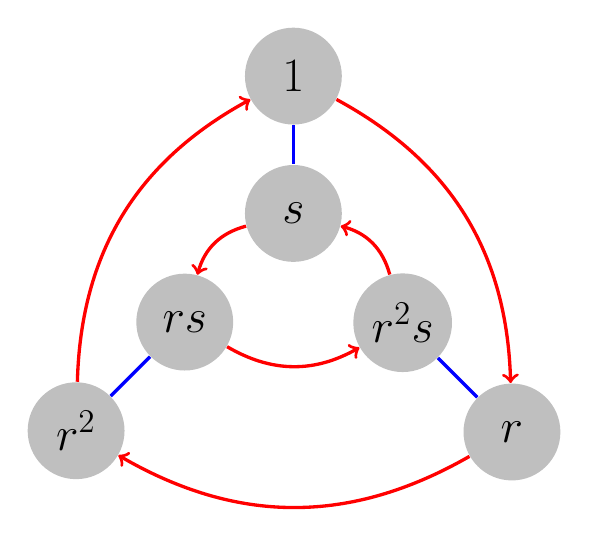
\begin{tikzpicture}[ele/.style = {circle, minimum size = 35pt, fill = lightgray, font = \LARGE},
  node distance = 0.50cm and 0.50cm,
  op2/.style = {-, blue, very thick},
  op3/.style = {->, red, very thick}]
  % inner
  \node (s) [ele] {$s$};
  \node (rs) [ele, below left = of s] {$rs$};
  \node (r2s) [ele, below right = of s] {$r^2s$};

  \path (s) edge[op3, bend right] (rs)
		(rs) edge[op3, bend right] (r2s)
		(r2s) edge[op3, bend right] (s);

  % outer
  \node (1) [ele, above = of s] {$1$};
  \node (r) [ele, below right = of r2s] {$r$};
  \node (r2) [ele, below left = of rs] {$r^2$};

  \path (1) edge[op3, bend left] (r)
		(r) edge[op3, bend left] (r2)
		(r2) edge[op3, bend left] (1);

  % join
  \path (1) edge[op2] (s)
		(r) edge[op2] (r2s)
		(r2) edge[op2] (rs);
\end{tikzpicture}
\end{document}

